\chapter{Зарождение, рост и кинетика превращения}

\section{Гомогенное зарождение}

Пересыщенный раствор метастабилен (глава~2): гидрид выгоднее, но его ещё нужно создать. Пусть в растворе
флуктуацией возник шарик новой фазы радиуса $r$. Объём даёт выигрыш $\Delta g$ на единицу объёма (химическая
движущая сила минус упругая энергия несоответствия), а поверхность стоит $\gamma$ на единицу площади:
\begin{equation}
\Delta G(r) = -\tfrac43\pi r^3\,\Delta g + 4\pi r^2\,\gamma .
\end{equation}
При малых $r$ побеждает поверхность ($r^2$), при больших --- объём ($r^3$). Функция имеет максимум
(рис.~\ref{fig:f6_cnt}):
\begin{keyf}[Критический зародыш]
\[
r^* = \frac{2\gamma}{\Delta g},\qquad \Delta G^* = \frac{16\pi}{3}\,\frac{\gamma^3}{\Delta g^2}.
\]
\end{keyf}
Зародыши меньше $r^*$ растворяются чаще, чем растут; больше $r^*$ --- растут. Барьер $\Delta G^*$ обратно
пропорционален \emph{квадрату} движущей силы. Вдвое большее пересыщение снижает барьер вчетверо.

\begin{figure}[htbp]\centering
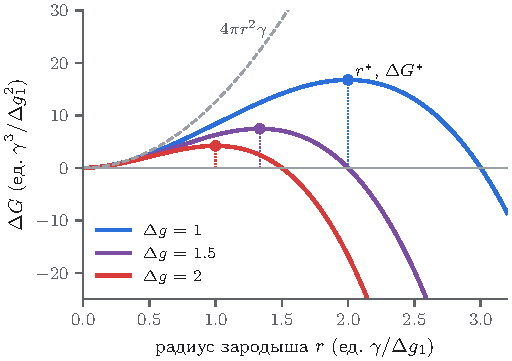
\includegraphics[width=0.6\linewidth]{f6_cnt}
\caption{Энергия зародыша от радиуса при трёх движущих силах. Точки --- критический радиус и барьер; с ростом
$\Delta g$ они быстро уменьшаются. Пунктир --- вклад поверхности.}
\label{fig:f6_cnt}
\end{figure}

\begin{zrbox}
Упругая энергия несоответствия $w$ вычитается из химической движущей силы: $\Delta g = \Delta g_{\text{хим}} - w$.
Если $w$ съедает большую часть $\Delta g_{\text{хим}}$, барьер огромен, и выпадения нет, пока раствор не пересытится
настолько, что $\Delta g_{\text{хим}}$ заметно превысит $w$. Это вторая сторона гистерезиса TSSD--TSSP из главы~2:
линия выпадения лежит там, где оставшаяся движущая сила $\Delta g_{\text{хим}} - w$ уже даёт заметную скорость
зарождения.
\end{zrbox}

\section{Скорость зарождения и С-кривые}

Число зародышей, появляющихся в единице объёма за единицу времени,
\begin{equation}
\dot N = N_s\,Z\,\beta^*\,\exp\Bigl(-\frac{\Delta G^*}{k_BT}\Bigr),
\end{equation}
где $N_s$ --- число мест для зарождения, $\beta^*$ --- частота присоединения атомов к критическому зародышу
(она пропорциональна $D$, то есть $e^{-Q/RT}$), $Z\sim0.01$--$0.1$ --- множитель Зельдовича (доля зародышей на
вершине барьера, которые всё-таки вырастут).

Два множителя тянут в разные стороны (рис.~\ref{fig:f6_rate}а). С переохлаждением движущая сила растёт, барьер
падает, и $e^{-\Delta G^*/kT}$ взлетает --- от нуля у $T_e$. Но с понижением температуры падает подвижность
$e^{-Q/RT}$. Их произведение имеет максимум. Если к скорости зарождения добавить скорость роста, получится время,
за которое превратится заданная доля, --- кривая в форме буквы С с «носом» на диаграмме
температура--время--превращение (рис.~\ref{fig:f6_rate}б).

\fig{f6_rate}{а) Скорость зарождения (чёрная) как произведение множителя барьера (красный, растёт с
переохлаждением) и подвижности (синий, падает при охлаждении). б) С-кривые начала (1\,\%) и конца (99\,\%)
превращения из тех же скоростей зарождения и роста (схема). Быстрее всего превращение идёт у «носа».}

\begin{idea}
Почему зарождение такое «пороговое»? Барьер стоит в показателе экспоненты и обычно в десятки $k_BT$. Если
$\Delta G^*/k_BT = 50$, то уменьшение барьера всего на 10\,\% (5$k_BT$) ускоряет зарождение в $e^5\approx150$ раз.
Поэтому при охлаждении зарождение почти не идёт, а затем в узком интервале температур начинается лавинообразно ---
это и видно как линия TSSP.
\end{idea}

\section{Неоднородное зарождение}

В реальном металле зародыш почти всегда появляется не в идеальном объёме, а на дефекте, который отдаёт часть своей
энергии. На границе зерна зародыш-линза заменяет кусок границы площадью $\pi a^2$ с энергией $\gamma_{\alpha\alpha}$
(рис.~\ref{fig:f6_het}а). Равновесие натяжений в точке стыка: $\gamma_{\alpha\alpha} = 2\gamma_{\alpha\beta}\cos\theta$.
Барьер уменьшается в $S(\theta)$ раз:
\begin{equation}
\frac{\Delta G^*_{\text{гр}}}{\Delta G^*_{\text{гом}}} = S(\theta) = \tfrac12(2+\cos\theta)(1-\cos\theta)^2 .
\end{equation}
Чем выше энергия границы по отношению к межфазной, тем меньше барьер (рис.~\ref{fig:f6_het}б). Ещё выгоднее
стыки трёх зёрен и их вершины. Мест на границах меньше, чем в объёме, но при малых переохлаждениях выигрыш в
барьере важнее числа мест.

\fig{f6_het}{а) Зародыш-линза на границе зерна; натяжения уравновешены при $\gamma_{\alpha\alpha} =
2\gamma_{\alpha\beta}\cos\theta$. б) Множитель барьера $S$ от отношения энергий границы и межфазной поверхности.}

Другие места неоднородного зарождения:
\begin{itemize}
\item \textbf{дислокации}: в растянутой области под краевой дислокацией несоответствие гидрида частично
  «скомпенсировано», и туда стекается водород (главы~3, 4);
\item \textbf{следы старых гидридов}: дислокационные петли и остаточная пластическая деформация после растворения
  (эффект памяти, глава~7);
\item \textbf{торцы уже растущих пластинок} --- там матрица растянута (глава~5).
\end{itemize}

\section{Форма зародыша}

Барьер для шара --- лишь приближение. Если межфазная энергия анизотропна (когерентная грань дешёвая, торцы
дорогие), а упругая энергия минимальна для тонкой пластинки (глава~5), выгоднее зародыш-диск. Для диска радиуса $a$
и толщины $2c$ с дешёвыми широкими гранями $\gamma_1$ и дорогими торцами $\gamma_2$ выигрыш тем больше, чем
сильнее $\gamma_2/\gamma_1$ и чем выгоднее тонкая форма упруго. Поэтому уже на стадии зарождения гидрид ---
тонкий когерентный диск на плоскости с наименьшей упругой энергией.

\section{Зарождение под напряжением}

Нагрузка добавляет к движущей силе работу $\sigma^A:\eps^*$ на единицу объёма гидрида (глава~5). Насколько это
сдвигает температуру выпадения? На линии выпадения при концентрации $C$ раствор пересыщен на
$RT\ln(C/C_e(T))$, а $C_e = Ae^{-Q/RT}$. Если работа нагрузки на моль водорода $W_\sigma = \sigma\eps^*V$
добавляется к движущей силе, то для той же скорости зарождения достаточно меньшего пересыщения, и выпадение
начнётся раньше на
\begin{keyf}[Сдвиг температуры выпадения]
\[
\delta T \approx \frac{T\,W_\sigma}{Q} = \frac{T\,\sigma\,\eps^*\,V}{Q}.
\]
\end{keyf}
Для гидрида ($T\approx580$~К, $\eps^* = 0.072$, $V = 10^{-5}$~м$^3$/моль H, $Q\approx32$~кДж/моль по наклону TSSP)
получается $\delta T/\sigma\approx0.013$~К/МПа. По измерениям на Zr--2.5Nb (Vizca\'{\i}no и др., 2014) сдвиг около
0.08~К/МПа --- в шесть раз больше. Значит, внешнее напряжение действует на зародыш сильнее, чем работа на его
среднем несоответствии. Возможные причины: концентрация напряжений у дефектов, где идёт зарождение;
пластичность; многоступенчатая природа зарождения. Это открытый вопрос, и в модели он отражён отдельным
параметром связи напряжений с зарождением.

\begin{figure}[htbp]\centering
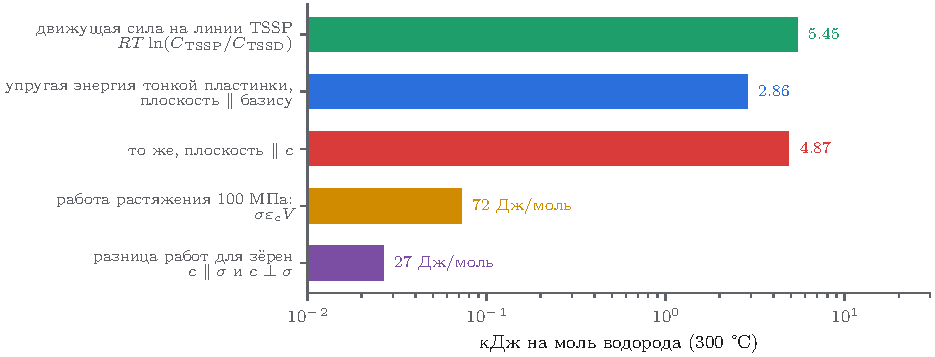
\includegraphics[width=0.85\linewidth]{f6_budget}
\caption{Энергетический бюджет выпадения гидрида на моль водорода при 300\degC{} для Э635 (логарифмическая шкала):
движущая сила на линии выпадения, упругая энергия тонкой пластинки на базисе и вдоль оси $c$, работа окружного
напряжения 100~МПа и разница этой работы между самым выгодным и самым невыгодным зерном.}
\label{fig:f6_budget}
\end{figure}

\begin{zrbox}
Почему крошечная работа решает ориентацию (рис.~\ref{fig:f6_budget})? После вычета упругой энергии у зародыша
остаётся $\Delta g\approx5.5-2.9\approx2.6$~кДж/моль~H. Работа 100~МПа --- 72~Дж/моль, то есть 2.8\,\% от этого
остатка. Барьер $\propto1/\Delta g^2$ уменьшается на $\approx5.5\,\%$. При барьере $50\,k_BT$ это $2.8\,k_BT$,
и скорость зарождения растёт примерно в 15 раз. Даже разница между зёрнами (27~Дж/моль) меняет скорость
примерно в 2.8 раза. В конкуренции зародышей такие множители решают, какие пластинки появятся первыми и заберут
водород.
\end{zrbox}

\section{Рост}

Зародыш, перешедший барьер, растёт. Гидрид богаче водородом, чем раствор, поэтому вокруг растущей пластинки
образуется обеднённая зона (рис.~\ref{fig:f6_growth}а). На границе --- равновесная концентрация $c_e$, вдали ---
исходная $c_0$. Если рост ограничен подводом водорода, граница движется со скоростью
\[
v = \frac{D}{c_\beta-c_e}\left.\frac{\partial c}{\partial x}\right|_{\text{гр}}\sim\frac{D}{c_\beta-c_e}\,\frac{c_0-c_e}{\sqrt{Dt}} .
\]
\begin{itemize}
\item \textbf{утолщение} широкой грани идёт по закону $\propto\sqrt{Dt}$: обеднённая зона перед ней расширяется, и
  подвод слабеет;
\item \textbf{удлинение} торца идёт с постоянной скоростью $\propto D(c_0-c_e)/r_{\text{торца}}$: острый торец всё
  время встречает свежий пересыщенный раствор (рис.~\ref{fig:f6_growth}б).
\end{itemize}

\fig{f6_growth}{а) Профиль концентрации у растущей пластинки: внутри --- состав гидрида $c_\beta$, на границе ---
равновесие $c_e$, вдали --- пересыщение $c_0$; обеднённая зона шириной $\sim\sqrt{Dt}$. б) Толщина растёт как
$\sqrt t$, длина --- линейно.}

Поэтому пластинки становятся всё более тонкими и длинными. Если рост ограничен не диффузией, а перестройкой
решётки на границе (\emph{рост, контролируемый границей}), скорость $v = M\,\Delta g$ определяется подвижностью
границы $M$ и не зависит от времени.

\section{Кинетика превращения в целом}

Если зародыши появляются со скоростью $\dot N$, а растут со скоростью $v$, то доля превращённого объёма $f(t)$
описывается уравнением Колмогорова--Джонсона--Мела--Аврами:
\begin{keyf}[Уравнение Аврами]
\[
f(t) = 1 - \exp\bigl(-(kt)^n\bigr).
\]
\end{keyf}
Вывод изящен. Сначала посчитаем «расширенный» объём, как если бы зёрна росли сквозь друг друга, не замечая
соседей: $f_{\text{расш}} = \int_0^t\dot N\,\tfrac43\pi v^3(t-\tau)^3\dd\tau\propto t^4$. Реальный прирост --- только
та часть, что попадает в ещё не превращённый объём: $\dd f = (1-f)\,\dd f_{\text{расш}}$. Отсюда
$f = 1-e^{-f_{\text{расш}}}$. Показатель $n$ говорит о механизме: 4 --- постоянное зарождение и трёхмерный рост,
3 --- все зародыши сразу, меньше --- рост в одном или двух измерениях или под контролем диффузии
(рис.~\ref{fig:f6_jmak}).

\fig{f6_jmak}{а) Кинетика Аврами при разных показателях $n$. б) В координатах $\ln(-\ln(1-f))$ против $\ln t$ ---
прямые с наклоном $n$; так показатель находят из опыта.}

\section{Огрубление и эффект Гиббса--Томсона}

У маленькой частицы велика доля поверхности, и её энергия на атом выше. Поэтому раствор вокруг неё равновесен
при большей концентрации:
\begin{equation}
c_r = c_\infty\exp\Bigl(\frac{2\gamma V}{rRT}\Bigr).
\end{equation}
Для гидрида при 300\degC{} и $\gamma=0.2$~Дж/м$^2$ частица радиусом 10~нм равновесна с раствором на 9\,\% богаче, чем
большая, а радиусом 1~нм --- вдвое (рис.~\ref{fig:f6_gt}). Водород течёт от мелких частиц к крупным: мелкие
растворяются, крупные растут. Это \textbf{огрубление} (созревание по Оствальду). Средний размер растёт как
$\bar r^3 - \bar r_0^3\propto t$ (теория Лифшица--Слёзова--Вагнера).

\begin{figure}[htbp]\centering
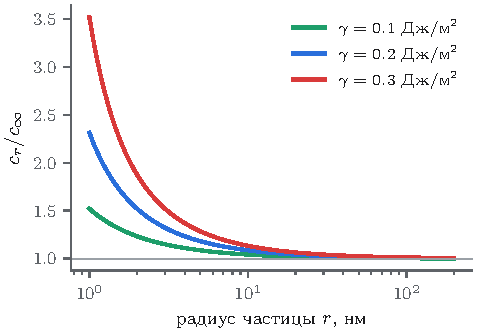
\includegraphics[width=0.58\linewidth]{f6_gt}
\caption{Эффект Гиббса--Томсона для гидрида при 300\degC: во сколько раз растворимость у частицы радиуса $r$ выше,
чем у плоской границы, при трёх энергиях межфазной границы.}
\label{fig:f6_gt}
\end{figure}

\begin{zrbox}
Для гидридов огрубление важно при выдержках у высоких температур: мелкие пластинки растворяются в пользу крупных.
Те же соображения объясняют, почему при нагреве первыми растворяются мелкие гидриды. А те, что остались
нерастворёнными на максимуме температуры, --- самые крупные. Они переживают цикл и задают, где выпадут новые
пластинки при охлаждении.
\end{zrbox}

\begin{exercise}
Выведите $r^*$ и $\Delta G^*$, приравняв нулю производную $\Delta G(r)$. Как изменится $\Delta G^*$, если движущая
сила уменьшится на 20\,\%?
\end{exercise}

\begin{exercise}
Покажите, что для линзы на границе зерна объём и площадь выражаются через объём шара того же радиуса кривизны и
множитель $S(\theta)$, и получите формулу $S(\theta)$.
\end{exercise}

\begin{exercise}
По формуле сдвига температуры выпадения оцените $\delta T$ для нагрузки 150~МПа. Сравните с шириной полосы гистерезиса
TSSD--TSSP.
\end{exercise}

\begin{exercise}
Выведите уравнение Аврами для случая, когда все зародыши появились в момент $t=0$ с плотностью $N$ и растут
трёхмерно со скоростью $v$. Какой получится показатель $n$?
\end{exercise}
